\documentclass[12pt, titlepage, a4paper]{article}
\usepackage[utf8]{inputenc}
\usepackage{changepage}
\usepackage{prftree}
\usepackage{amssymb}
\usepackage{amsmath}
\usepackage{enumitem} 
\usepackage{graphicx}
\usepackage{wrapfig}
\usepackage[spanish]{babel}
\usepackage{amsthm}
\usepackage{bussproofs}
\usepackage{bm}
\usepackage{url}
\usepackage{hyperref}
\usepackage{dirtytalk}
\usepackage{xcolor}

\usepackage{titlesec}
\usepackage[export]{adjustbox}

\setcounter{secnumdepth}{4}

\titleformat{\paragraph}
{\normalfont\normalsize\bfseries}{\theparagraph}{1em}{}
\titlespacing*{\paragraph}
{0pt}{3.25ex plus 1ex minus .2ex}{1.5ex plus .2ex}


\usepackage[a4paper, total={6in, 8in}]{geometry}


\usepackage{amsmath}
\usepackage{algorithm}
\usepackage{algorithmic}

\newcommand{\high}[2]{{\color{#1} \textbf{#2}}}

\title{Introducción a la Inteligencia Artificial \\
Trabajo Práctico 2: Ontologías }
\author{Agustín Fernández Bergé y Ramiro Gatto}
\date{14/04/2025}

\begin{document}
\maketitle
    

\section{Introducción}
La idea de este trabajo es modelar una ontología 
(en Protege) sobre lenguajes de  
programación, en la cual se represente las características que estos 
poseen. El principal uso de la misma es permitir ayudar a un programador
a elegir un lenguaje apropiado para un proyecto según sus necesidades. 

\section{Pasos a Seguir}
Para guiarnos en la creación de la ontología seguimos el \say{Pipeline} que 
vimos en clase, el cual consiste en lo siguientes pasos:

\begin{enumerate}
    \item {\textbf{Determinar dominio y alcance}\\
           En esta primera instancia nos planteamos preguntas que deben 
           ser respondidas por la ontología. Estas deben estar relacionadas 
           con: el dominio que cubre, el propósito de la misma y para que 
           consultas da solución. Nosotros propusimos las siguientes:
           \begin{itemize}
                \item {\say{¿Qué lenguajes funcionales tienen tipado estático y fuerte?}}
                \item {\say{¿Qué lenguajes tienen recolector de basura?}}
                \item {\say{¿Qué lenguajes son multiparadigmas?}} 
                \item {\say{¿Qué lenguajes son aptos para programar de forma concurrente?}}
           \end{itemize}}
    \newpage
    \item {\textbf{Analizar Reuso}\\
           Para poder facilitar la creación de más clases y/o tener mas 
           idea de que características usar en la ontología, una 
           forma seria viendo otras ontología ya creadas.

           En nuestro caso intentamos seguir el enfoque de Peter Van Roy\cite{vanroy} que
           asocia lenguajes de programación con uno o más paradigmas de programación
           y a su vez asocia paradigmas de programación con una o más conceptos de programación.\\

           \begin{center}
            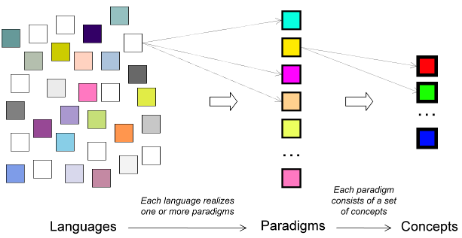
\includegraphics[scale=0.75]{Imagenes/lenguajesParadigmasConceptos.png}
           \end{center}

           Sin embargo definir un paradigma puramente por los conceptos es complicado y puede terminar en muchos
           paradigmas diferentes que difieren solo en un concepto. Separar demasiado los paradigmas siguiendo este enfoque 
           puede complicar mucho el diseño de la ontología y puede hacerla demasiado general como para los objetivos que nos propusimos.

           Aun asi no abandonamos este enfoque del todo, simplemente decidimos separar los conceptos (nosotros lo llamamos
           características) de los paradigmas de programación.
           }
    \item {\textbf{Enumerar términos}\\
           En base al lo pensado en los apartados anteriores se comenzó a 
           enumerar los elementos que van a aparecer en la ontología.
           Pensando:
           \begin{itemize}
            \item {¿De qué términos necesitamos hablar?}
            \item {¿Propiedades que poseen esos términos?}
            \item {¿Qué queremos decir acerca de esos términos?} 
           \end{itemize}
           Para esta ontología surgieron los siguientes (entre muchos mas):
           \begin{itemize}
            \item {Lenguajes: C, C++, Python, Haskell, ...}
            \item {Características: paradigma, gestor de memoria, forma de ejecución, ...}
           \end{itemize}}
    \item {\textbf{Definición de clases y jerarquía}\\
           Para poder definir las clases nos guiamos por la idea de que 
           una clase es una colección de elementos con propiedades
           similares (Ejemplos de clases en esta ontología serian los 
           Lenguajes y Programas).\\

           Ademas, también se tuvo en consideración la idea 
           de subclases y superclases (Como puede ser en el caso 
           de las Características)}
    \item {\textbf{Definición propiedades de las clases (slots)}\\
           En esta sección es donde pensamos las propiedades (slots) 
           que van a tener las instancia de una clase y como 
           se van a relacionar con las instancias de otra clase. 
           Un ejemplo seria:
           \begin{enumerate}
                \item {Cada Programa fue escrito en algún Lenguaje}
                \item {Cada Lenguaje tiene algún paradigma}
                \item {Cada Lenguaje tiene una forma de gestión de memoria}
                \item {Cada Lenguaje tiene una forma de ejecución}
                \item Cada lenguaje tiene varias características de su sistema de tipo
                \begin{itemize}
                    \item {El sistema de tipo puede ser fuerte o débil}
                    \item {El sistema de tipo puede tener tipado estático o dinámico}
                    \item {La Declaración de tipos puede ser implícita o explícita}
                \end{itemize}
           \end{enumerate}}
    \item {\textbf{Restricción de Propiedades}\\
          En esta sección, se establecieron los posibles valores de 
          los slots teniendo se: 
          \begin{itemize}
            \item {Un lenguaje de programación es una instancia de Lenguaje}
            \item {Un programa puede ser escrito por multiples lenguajes}
            \item {Los Lenguaje tienen una sola forma de gestión de memoria}
            \item {Los Lenguajes tienen una sola forma de ejecución}
            \item {Los Lenguajes pueden tener multiples paradigmas}
            \item {El sistema de tipos puede ser fuerte o débil, pero no 
                ambos a la vez}
            \item {El sistema de tipos puede ser estático o dinámico, pero no
                ambos a la vez}
            \item {La declaración de tipos puede ser implícita, explícita o ambas al mismo tiempo}
          \end{itemize}
          }
    \item {\textbf{Crear instancia}\\
         Para esta sección simplemente creamos las instancia en las 
         distintas clases y le asignamos los valores según las slots.\\ 
         Un ejemplo de esto seria, en Lenguaje agregamos la 
         instancia \textbf{C}, en GestionMemoria \textbf{Manual}. 
         Luego podemos relacionar \textbf{C} y \textbf{Manual} mediante la 
         propiedad \textbf{tieneGestionMemoria}}
\end{enumerate}

\section{Conceptos representados}
En la ontología final representamos los siguientes conceptos
\begin{itemize}
    \item {Característica, cualidades que cumplen los lenguajes de programación, 
        nosotros optamos pos usar:
        \begin{itemize}
            \item {Gestión de memoria, representa las forma en las que los 
                lenguaje manejan el uso de la memoria}
            \item {Forma de ejecución, }
            \item {Paradigma, con paradigma nos referimos al
                enfoque para crear programs}
            \item {Sistema de tipo, esta clasificación se divide en 3 mas
                Chequeo de tipo (verificar que los tipos de datos 
                en un programa sean correctos), Declaración de tipo 
                (especificar explícitamente el tipo de una variable), 
                Seguridad de tipo (garantizar que las operaciones solo 
                se realicen entre datos de tipos compatibles)}
        \end{itemize}}
    \item {Lenguaje, hace referencia a todos los lenguajes de programación 
        que decidimos agregar}
    \item {LenguajeInteresnte, este es una clase definida (no primitiva) en la 
            la cual fue creada para probar el razonador, en esta solo se encentran 
            las instancias de lenguajes que cumplen una serie de restricciones 
            (posee al menos 3 paradigmas, posee recolector de basura y tiene 
            chequeo y seguridad de tipos)}
\end{itemize}

\noindent Quedándonos la siguiente ontología:
\begin{figure}[H]
    \centering
    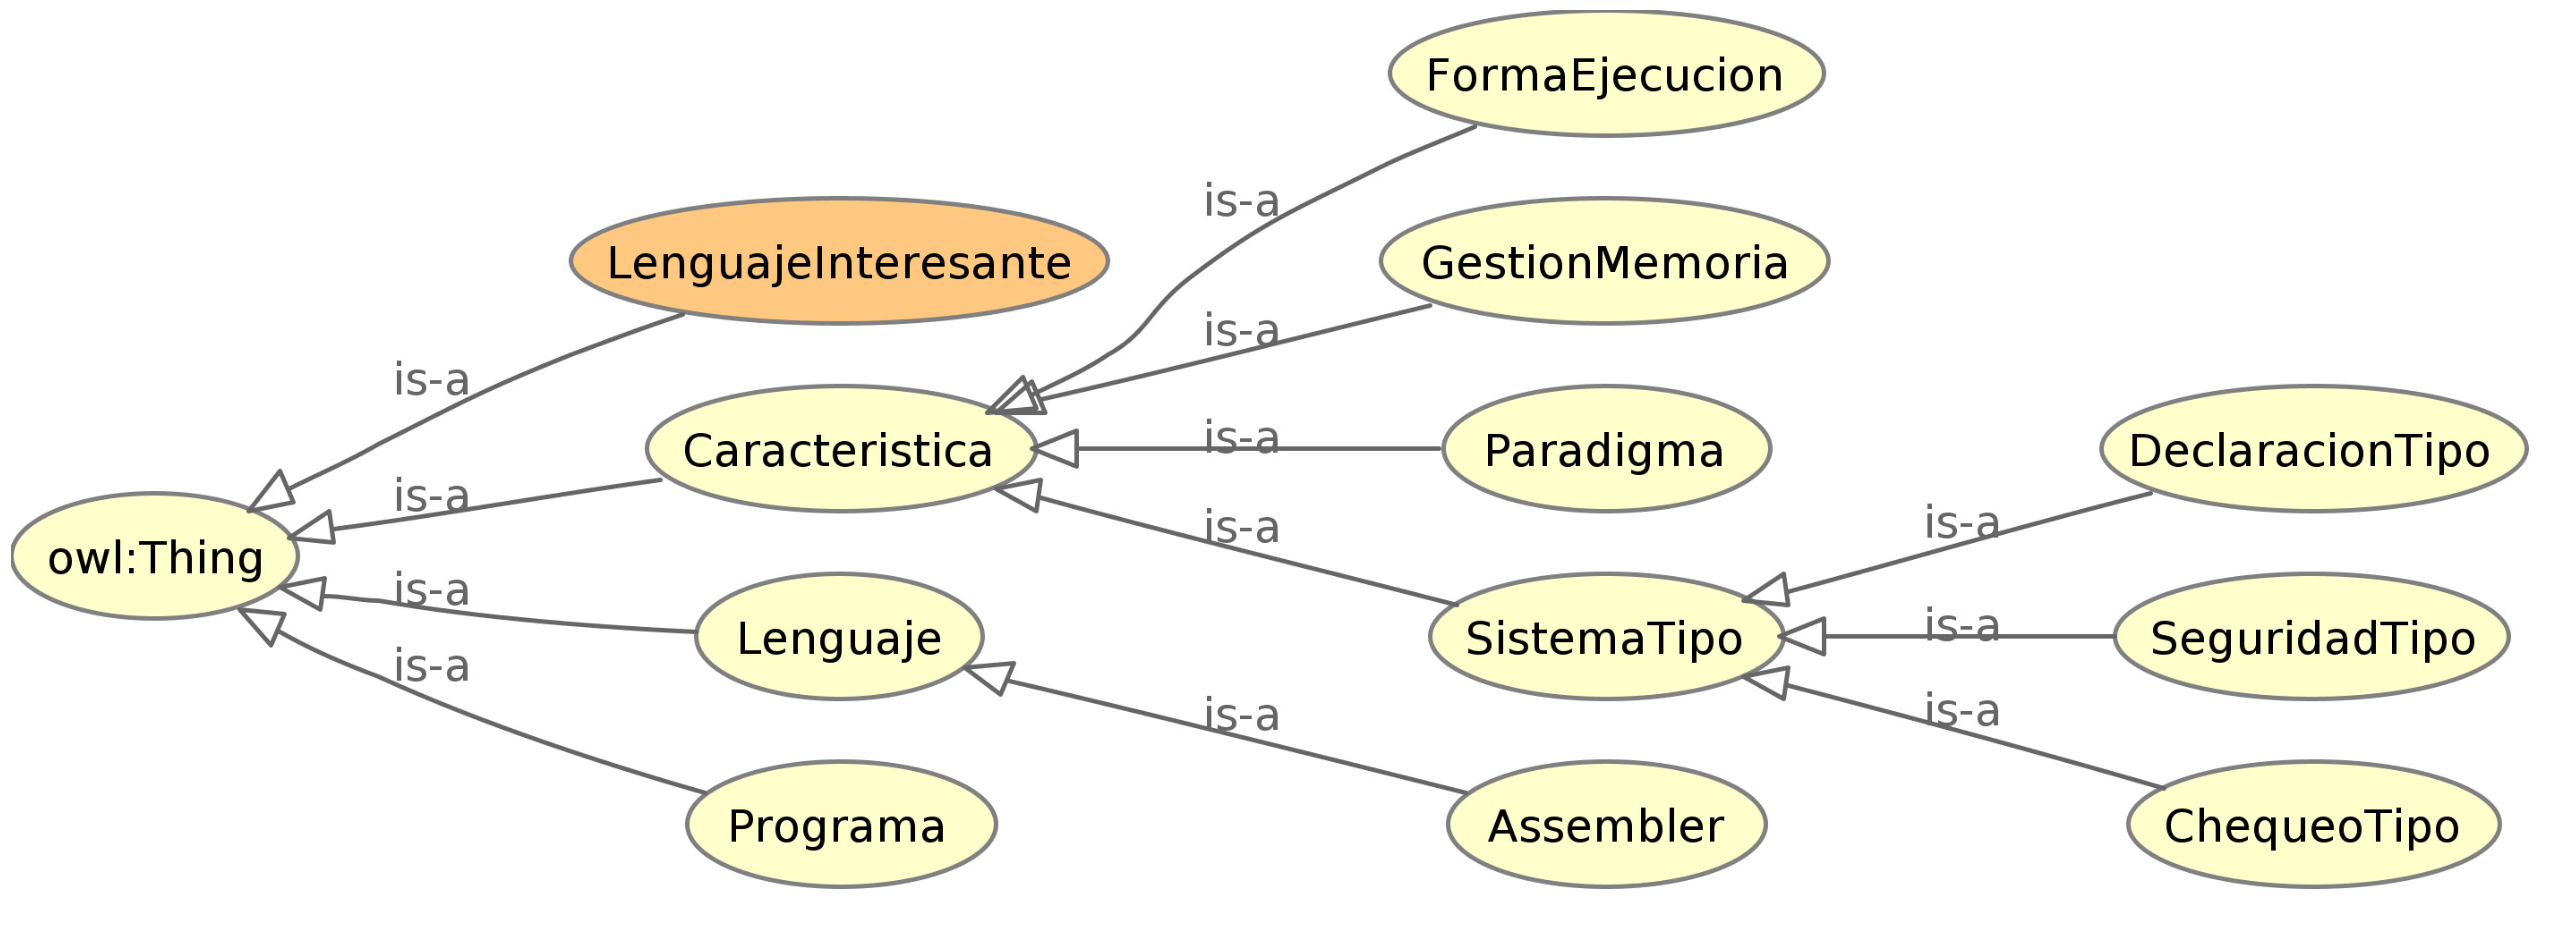
\includegraphics[width=.8\textwidth]{Imagenes/Ontologia.png}
    \caption{Ontología}
\end{figure}

\section{Instancias propuesta}
Las instancias nos quedaron de la siguiente forma:
\begin{figure}[H]
    \centering
    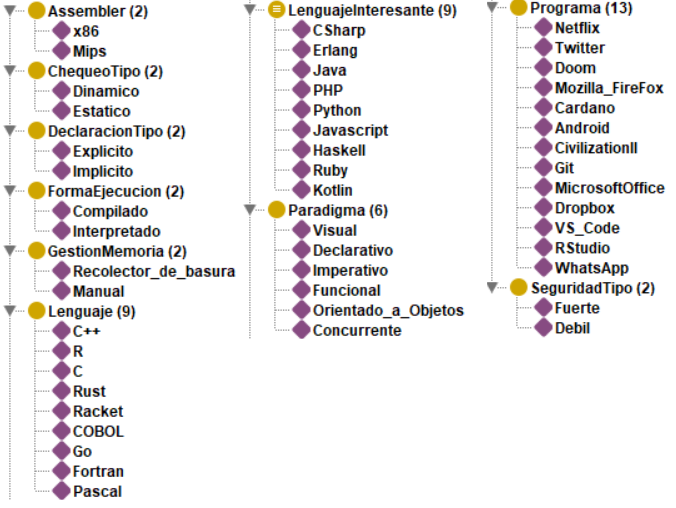
\includegraphics[width=.5\textwidth]{Imagenes/Instancias3.png}
    \caption{Instancia}
\end{figure}

En cuanto al temas de las relaciones tenemos las siguientes
\begin{figure}[H]
    \centering
    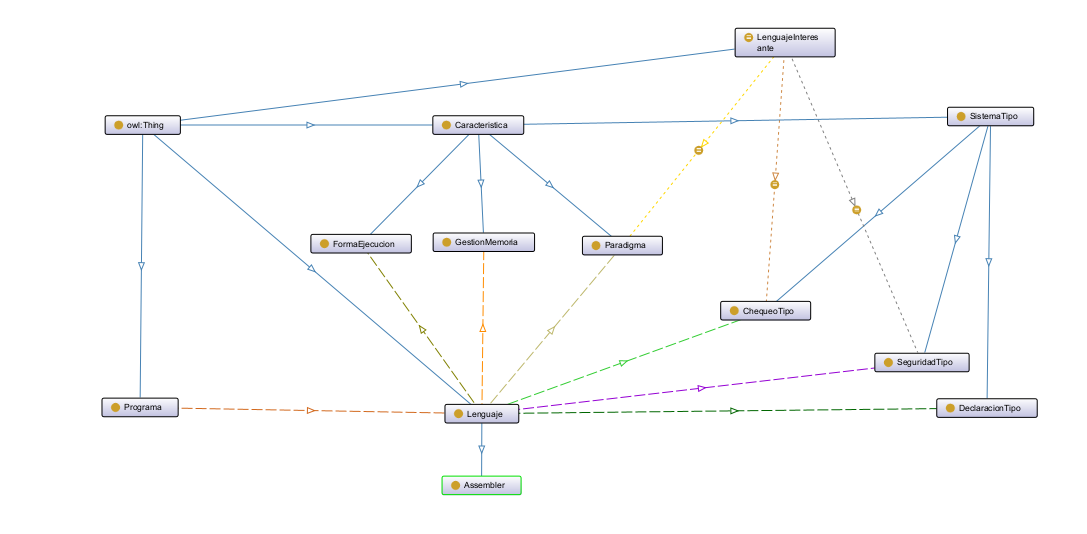
\includegraphics[width=.8\textwidth]{Imagenes/Relaciones3.png}
    \caption{Relaciones, las inversas no aparecen}
\end{figure}

\section{Resultados obtenidos con el razonador}
Para ver como funciona el razonador lo que hacemos es lo siguiente, 
definimos cada relación y su inversa. Cuando \say{Instanciamos} solo 
lo hacemos con las normales, no con la inversa. De esta forma el 
razonador infiere el tipo de la inversa.\\

La otra que hacemos es dejar que intuya solo el valor de la inversa, 
es decir si las instancias A y B se relaciona mediante la realización 
f (A $\rightarrow^f$ B) dejamos que el razonador haga la inversa 
(es decir, B $\rightarrow^{f^{-1}}$ A)

%Berge, no se que mas poner

\section{Consultas realizadas}
Para ver el resultado de las consultas vamos a probar con las 
preguntas que planteamos al momento de determinar el alcance y 
veamos si en efecto son correctas. Escribimos las consultas utilizando
\textbf{DL Query}.

\begin{description}
    \item[Pregunta:] ¿Qué lenguajes funcionales tienen tipado estático y fuerte?
    \item[Consulta:] (tieneParadigma \high{magenta}{value} Funcional) \high{cyan}{and} 
    (tieneSeguridadTipo \high{magenta}{value} Fuerte) \high{cyan}{and} 
    (tieneChequeoTipo \high{magenta}{value} Estatico)
    \item[Respuesta:] C++, CSharp, Fortran, Haskell, Java, Kotlin y Rust.\\
    
    \item[Pregunta:] ¿Qué lenguajes tienen recolector de basura?
    \item[Consulta:] tieneGestionMemoria \high{magenta}{value} Recolector\_de\_basura
    \item[Respuesta:] CSharp, Erlang, Go, Haskell, Java, Javascript, Kotlin, PHP, Python, Racket y Ruby.\\
    
    \item[Pregunta:] ¿Qué lenguajes son multiparadigmas?
    \item[Consulta:] tieneParadigma \high{magenta}{min} 2
    \item[Respuesta:] C++, COBOL, CSharp, Erlang, Fortran, Go, Haskell, Java, Javascript, Kotlin, PHP, Python, Racket, Ruby y Rust.\\
    
    \item[Pregunta:] ¿Qué lenguajes son aptos para programar de forma concurrente?
    \item[Consulta:] aptoParaProgramar \high{magenta}{value} Concurrente
    \item[Respuesta:] C++, CSharp, Erlang, Fortran, Go, Haskell, Java, Kotlin, Racket y Rust.\\
\end{description}

\section{Análisis del razonamiento del razonador}
Para esta sección veamoslo con algunas de las consultas de 
la seccion anterior anteriores.\\

Empecemos con: tieneGestionMemoria \high{magenta}{value} Recolector\_de\_basura\\
Si vemos la  respuesta que nos dan se ve que una de ellas es Haskell,
 entonces para responder porque da este resultado podemos ver la explicación, siendo esta. 
\begin{figure}[H]
    \centering
    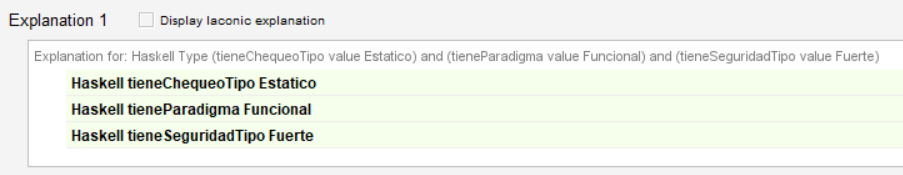
\includegraphics[width=.8\textwidth]{Imagenes/Explicacion1.png}
    \caption{}
\end{figure}
La cual nos dice que Recolector\_de\_basura se relacion con Haskell por medio de 
la relacion esGestionMemoriaDe y esta es inversa de tieneGestionMemoria por lo 
que el razonador puede inferir que Haskell se relaciona con Recolector\_de\_basura 
mediante tieneGestionMemoria (dando el resultado correcto)

\noindent Veamos ahora con: tieneParadigma \high{magenta}{min} 2\\
De la respuesta vemos que Rust es una de ellas, veamos el porque.\\
El razonamiento fue el siguiente:
\begin{figure}[H]
    \centering
    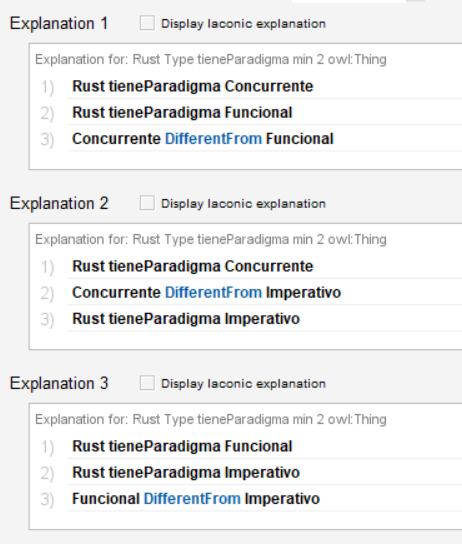
\includegraphics[width=.5\textwidth]{Imagenes/Explicacion2.png}
    \caption{}
\end{figure}
Donde en un inicio se tiene que Rust tiene 3 tipos paradigmas (distintos entre si). 
Lo que hace el razonador es verificar que haya al menos 2 distintos, y como 
los tres son distintos entre si, el razonador encuentra 3 justificaciones 
validas para dar a Rust como respuesta.

\section{Conclusion}
Además de intentar el ya mencionado enfoque de Peter Van Roy, surgieron otras
cuestiones durante la creación de la ontología.

\begin{itemize}
    \item Intentamos declarar los lenguajes como clases y las versiones de los mismos con instancias.
    Puede haber diferencias significativas entre versiones de un mismo lenguaje (ejemplo, Python 3.5 en adelante
    incluye tipado explicito opcional y C++11 incluye tipado dinámico). Pero por lo general una persona no busca elegir
    una versión especifica de un lenguaje, sino que elige el lenguaje en si y despues una version estable.  Además que
    la inclusión de las versiones de los lenguajes esta fuera del alcance que necesitamos para responder nuestras preguntas.
    \item Intentamos incluir como característica el nivel de abstracción del lenguaje (si es de bajo o alto nivel).
    El nivel de abstracción es un concepto relativo y no es fácil de definir sin conocer el lenguaje en si. C hasta hace no mucho
    era un lenguaje de alto nivel ya que proveía de conceptos structs y funciones recursivas parametrizadas. Sin embargo en la actualidad
    es considerado de bajo nivel debido a que no tiene características como un recolector de basura. Como el nivel de abstracción no es facilmente
    definible, decidimos no incluirlo como característica.   
\end{itemize}

\begin{thebibliography}{999}

    \bibitem{vanroy}
      Peter Van Roy. 
      \href{https://webperso.info.ucl.ac.be/~pvr/VanRoyChapter.pdf}{\emph{Programming Paradigms: What Every Programmer Should 
      Know}(PDF)}.
    
    \bibitem{comparacionPorTipo}
      Wikipedia, \href{https://en.wikipedia.org/wiki/List_of_programming_languages_by_type}{\emph{List of programming languages by type}}.
    
    \bibitem{comparacionPorSistemaTipo}
      Wikipedia, \href{https://en.wikipedia.org/wiki/Comparison_of_programming_languages_by_type_system}{\emph{Comparison of programming languages by type system}}.
    
    \bibitem{comparacionParadigma}
      Wikipedia, \href{https://en.wikipedia.org/wiki/Comparison_of_multi-paradigm_programming_languages}{\emph{Comparison of multi-paradigm programming languages}}.
    
    
\end{thebibliography}

\end{document}